\documentclass[11pt]{article}

\usepackage[margin=1in]{geometry}
\usepackage[utf8]{inputenc}
\usepackage[T1]{fontenc}
\usepackage{lmodern}
\usepackage{amsmath}
\usepackage{graphicx}
\usepackage{booktabs}
\usepackage{float}
\usepackage{caption}
\usepackage{hyperref}

\graphicspath{{../figures/}}

\setlength{\emergencystretch}{4em}

\title{Project 3 Report: Clustering, PCA and SVD on MovieLens Ratings}
\author{Lukas Anell}
\date{November 2026}

\begin{document}
\maketitle

\section*{Summary}

% TODO

\section*{Introduction}

% TODO

\section{Transforming Data}
\label{sec:s1}

% TODO

\subsection*{1(a) Most Rated Movies}

\begin{table}[H]
    \centering
    \begin{tabular}{lc}
        \toprule
        Movie                            & Users who rated it \\
        \midrule
        Forrest Gump (1994)              & 329                \\
        Shawshank Redemption, The (1994) & 317                \\
        Pulp Fiction (1994)              & 307                \\
        \bottomrule
    \end{tabular}
    \caption{The three movies rated by the most users (\texttt{src/section1.py}).}
    \label{tab:top_items}
\end{table}

\subsection*{1(b) Most Active Users}

\begin{table}[H]
    \centering
    \begin{tabular}{cc}
        \toprule
        \texttt{userId} & Movies rated \\
        \midrule
        414             & 2698         \\
        599             & 2478         \\
        474             & 2108         \\
        \bottomrule
    \end{tabular}
    \caption{The three users who rated the most movies (\texttt{src/section1.py}).}
    \label{tab:top_users}
\end{table}

\section{Clustering}
\label{sec:s2}

\subsection*{2(a) Inertia}

\begin{figure}[H]
    \centering
    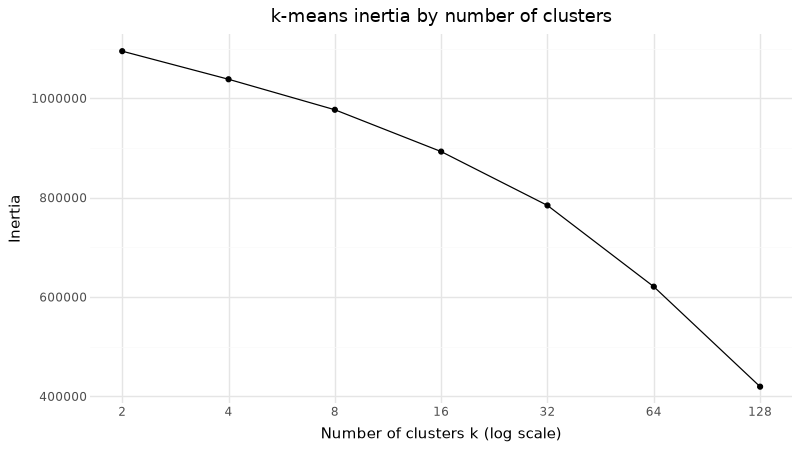
\includegraphics[width=0.8\linewidth]{inertia_vs_k.png}
    \caption{k-means inertia for $k = 2, 4, 8, 16, 32, 64, 128$ (log$_2$ x axis).}
    \label{fig:inertia}
\end{figure}

\subsection*{2(b) Choice of $k$}

% TODO

\subsection*{2(c) Top Movies per Cluster}

% TODO: recheck
\begin{table}[H]
    \centering
    \begin{tabular}{clcc}
        \toprule
        Cluster (users) & Movie                          & Raters & Mean rating \\
        \midrule
        0 (457)         & Shawshank Redemption, The (1994) & 207  & 4.40        \\
        & American History X (1998)      & 59     & 4.31        \\
        & Godfather: Part II, The (1974) & 49     & 4.27        \\
        \addlinespace
        1 (80)          & Shawshank Redemption, The (1994) & 64   & 4.57        \\
        & Platoon (1986)                 & 9      & 4.44        \\
        & Pulp Fiction (1994)            & 63     & 4.44        \\
        \addlinespace
        2 (15)          & Night on Earth (1991)          & 2      & 5.00        \\
        & Stranger Than Paradise (1984)  & 2      & 5.00        \\
        & Smoke (1995)                   & 2      & 4.75        \\
        \addlinespace
        3 (58)          & Bottle Rocket (1996)           & 6      & 4.75        \\
        & Lawrence of Arabia (1962)      & 17     & 4.74        \\
        & Touch of Evil (1958)           & 7      & 4.71        \\
        \bottomrule
    \end{tabular}
    \caption{Top three movies per cluster at $k = 4$, ranked by the mean of the non-zero ratings from users in the cluster, among movies rated by at least 10\% of the cluster's users. Ties in the mean are broken by the number of raters, then by \texttt{movieId}.}
    \label{tab:cluster_top}
\end{table}

% TODO

\section{Principal Component Analysis}
\label{sec:s3}

\subsection*{3(c) Movies by First Genre}

\begin{figure}[H]
    \centering
    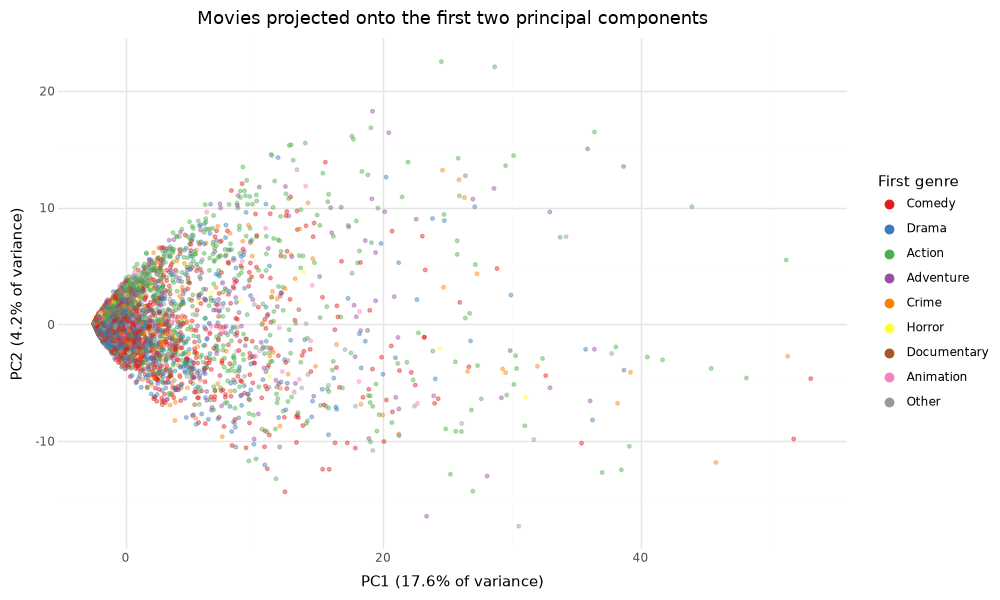
\includegraphics[width=\linewidth]{pca_movies_by_genre.png}
    \caption{The 9,724 movies projected onto the first two principal components of the user-mean-centered movie-by-user matrix, colored by first listed genre. The eight most frequent first genres are shown, and all others, including movies with no genre listed, are grouped as Other. Points are partly transparent.}
    \label{fig:pca}
\end{figure}

% TODO

\subsection*{3(d) Intrinsic Dimensionality}

% TODO

\section{Singular Value Decomposition}
\label{sec:s4}

\subsection*{4(a) Singular Values}

\begin{figure}[H]
    \centering
    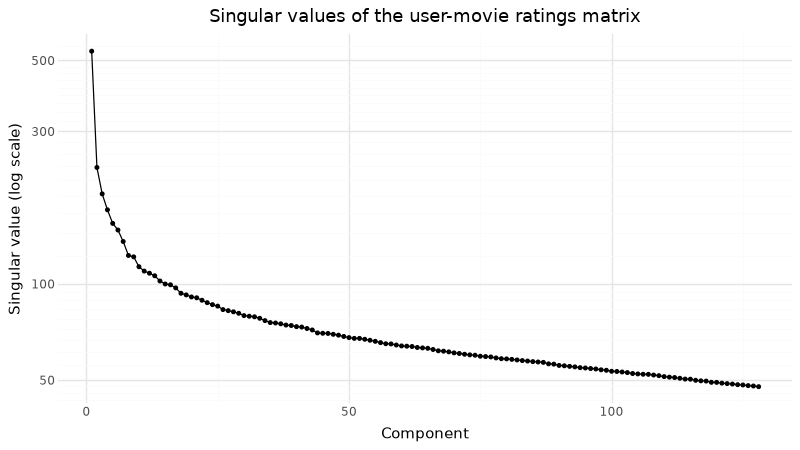
\includegraphics[width=0.8\linewidth]{svd_singular_values.png}
    \caption{The 128 largest singular values of the user-by-movie ratings matrix, without centering (log y axis).}
    \label{fig:singular}
\end{figure}

\subsection*{4(b) Explained Variance}

% TODO: recheck
\begin{table}[H]
    \centering
    \begin{tabular}{rcrc}
        \toprule
        $k$ & SVD variance explained & k-means inertia & k-means variance explained \\
        \midrule
        2   & 0.1728                 & 1,094,664       & 0.0940                     \\
        4   & 0.2219                 & 1,038,120       & 0.1408                     \\
        8   & 0.2870                 & 976,741         & 0.1916                     \\
        16  & 0.3636                 & 892,564         & 0.2613                     \\
        32  & 0.4619                 & 784,126         & 0.3510                     \\
        64  & 0.5894                 & 620,650         & 0.4863                     \\
        128 & 0.7475                 & 419,352         & 0.6529                     \\
        \bottomrule
    \end{tabular}
    \caption{Sum of \texttt{explained\_variance\_ratio\_} from a separate \texttt{TruncatedSVD} fit for each $k$, next to the k-means inertia for the same $k$. The last column is one minus the inertia divided by the total sum of squares about the column means (1,208,281), which puts k-means on the same scale as the SVD column.}
    \label{tab:variance}
\end{table}

% TODO

\subsection*{4(d) Users in the SVD Embedding}

\begin{figure}[H]
    \centering
    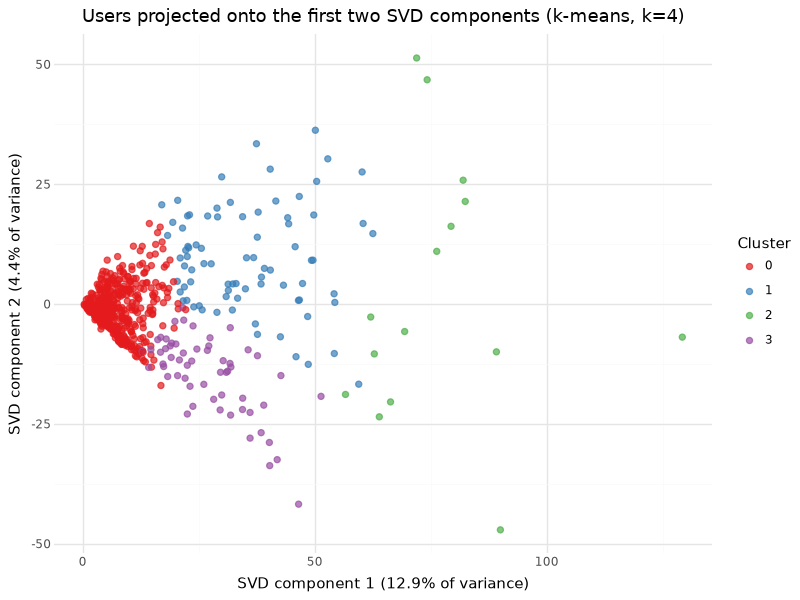
\includegraphics[width=0.8\linewidth]{svd_users_by_cluster.png}
    \caption{The 610 users projected onto the first two SVD components, colored by their $k = 4$ k-means cluster from Section~\ref{sec:s2}.}
    \label{fig:svd_users}
\end{figure}

% TODO

\section{Reflection}
\label{sec:reflection}

% TODO

\subsection{Something I Understand Differently Now}

\subsection{A Decision I Made}

\subsection{A Moment of Uncertainty}

\subsection{Looking Back}

\end{document}
